\section{Performance evaluation}
The SVM classifier implemented in the scikit-learn library uses a RBF kernel (equation \ref{eq:rbf}) while in OpenCV is possible to choose which kernel and eventually the degree of the model. 

\begin{equation} \label{eq:rbf}
    K(x,x') = \exp \left(\frac{||x-x'||^2}{2\sigma^2}\right)
\end{equation}

The scikit-learn classifier offers the best performances, in figure \ref{fig:confusion} is possible to see the confusion matrices for both this classifier and the RBF OpenCV one. 

\begin{figure}[h!t]
    \centering
    \begin{subfigure}{.4\textwidth}
        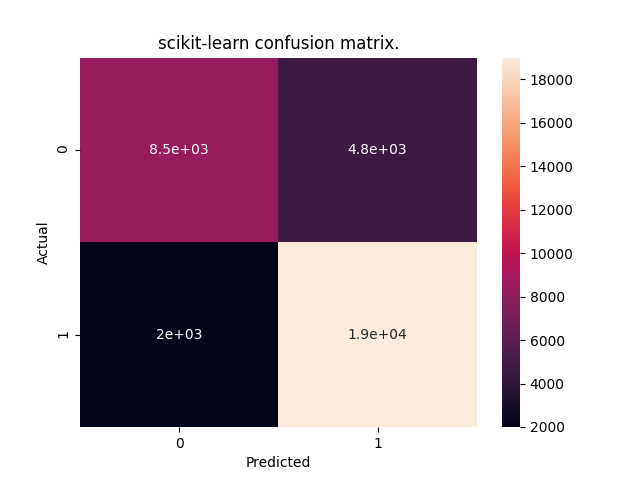
\includegraphics[scale=0.29]{images/confusion_skl.png}
        \caption{Confusion matrix for \textit{scikit-learn}.}
        \label{fig:confusion_skl}
    \end{subfigure}
    ~
    \begin{subfigure}{.4\textwidth}
        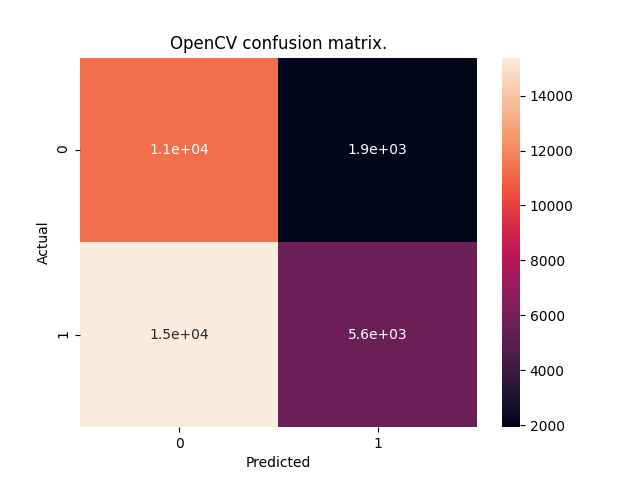
\includegraphics[scale=0.29]{images/confusion_cv2.png}
        \caption{Confusion matrix for \textit{scikit-learn}.}
        \label{fig:confusion_cv2}
    \end{subfigure}
    \caption{Confusion matrices.}
    \label{fig:confusion}
\end{figure}

The scores obtained are collected on table \ref{tab:scores}.

\begin{table}[h!t]
    \centering
    \caption{Scores for the classifiers.}
    \label{tab:scores}
    \begin{tabular}{lcc}
        & scikit & OpenCV \\
        Accuracy & 0.805 & 0.491 \\
        Precision & 0.814 & 0.421 \\
        Recall & 0.639 & 0.860 \\
        F1 & 0.358 & 0.283 \\
    \end{tabular}
\end{table}

In images \ref{fig:roc} are plotted the ROC curves for the scikit-learn SVM classifier and OpenCV ones with linear, 3-degree polynomial and RBF kernels. 

\begin{figure}[h!t]
    \centering
    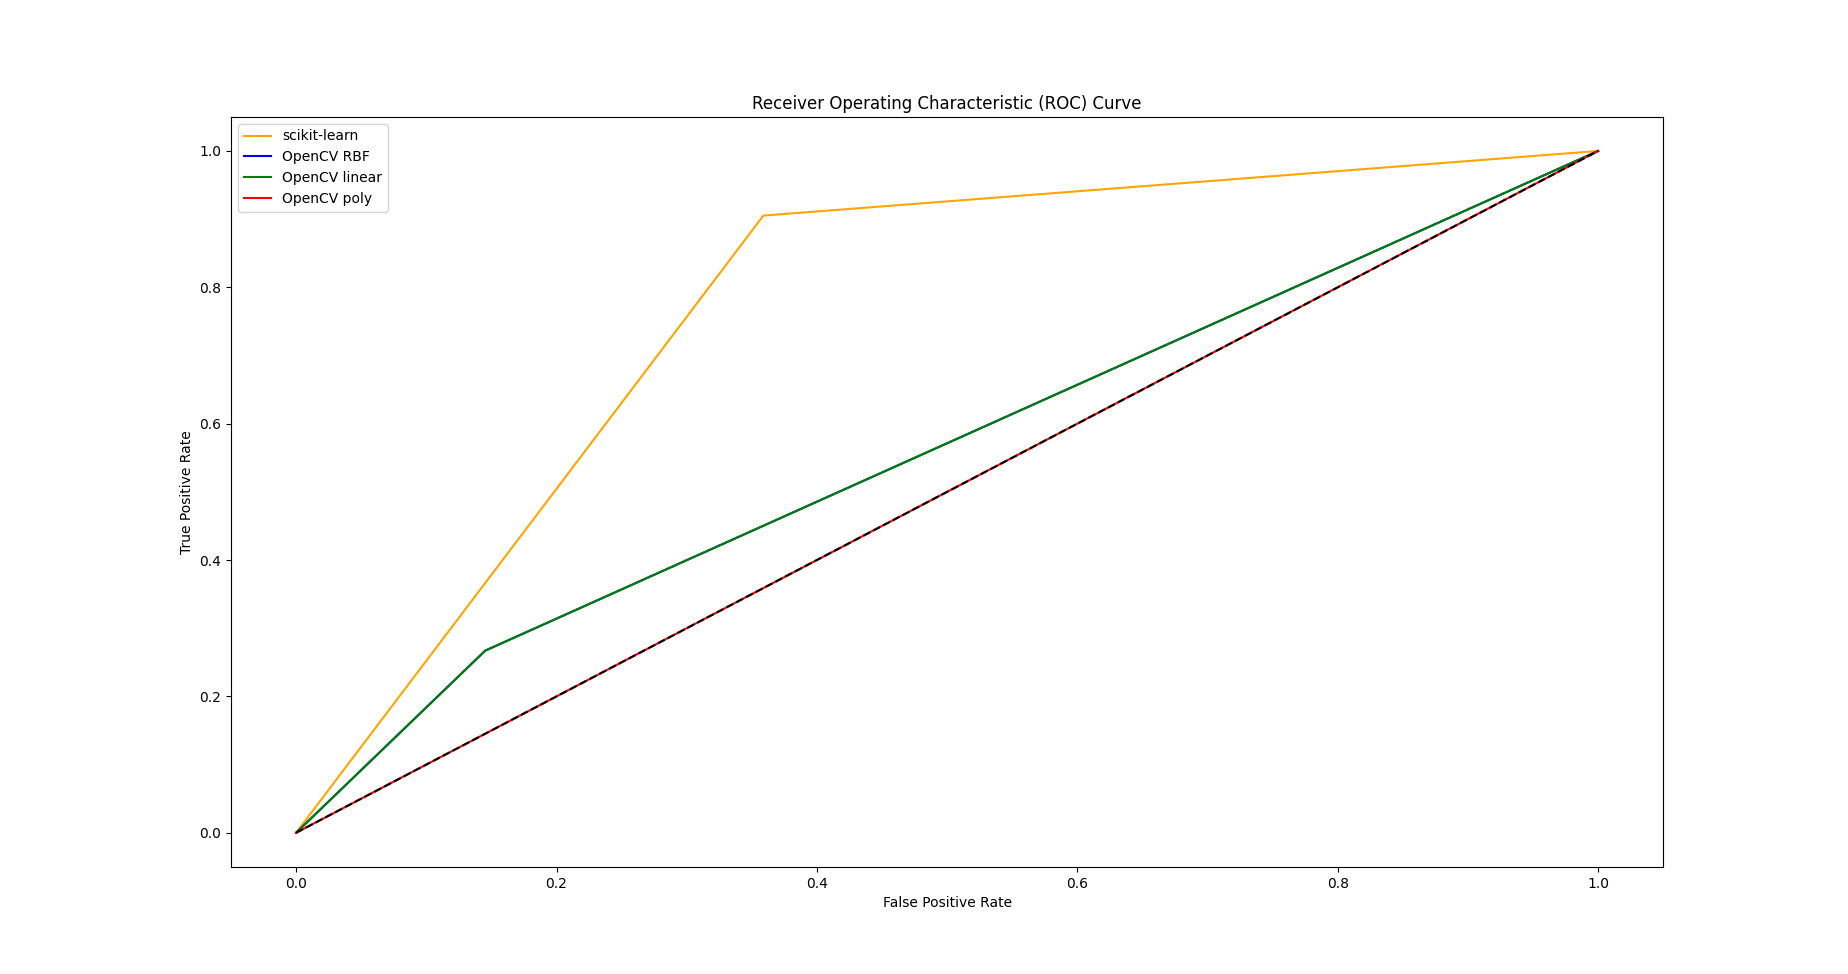
\includegraphics[scale=0.25]{images/roc.png}
    \caption{ROC.}
    \label{fig:roc}
\end{figure}

The polynomial one has terrible performances, is like throwing chances \footnote{has an AUC of 0.5}, while the linear and rbf ones overlap each other with quite better performances.
Still the best performing one is the scikit-learn with a rbf kernel, on table \ref{tab:auc} are displayed the AUCs.

\begin{table}[h!t]
    \centering
    \caption{Scores for the classifiers.}
    \label{tab:auc}
    \begin{tabular}{lcc}
        & scikit & OpenCV \\
        AUC & 0.774 & 0.560 \\
    \end{tabular}
\end{table}

On figure \ref{fig:det} are plotted the DET curves for only the scikit classifier and the OpenCV one, both with rbf kernel. 

\begin{figure}[h!t]
    \centering
    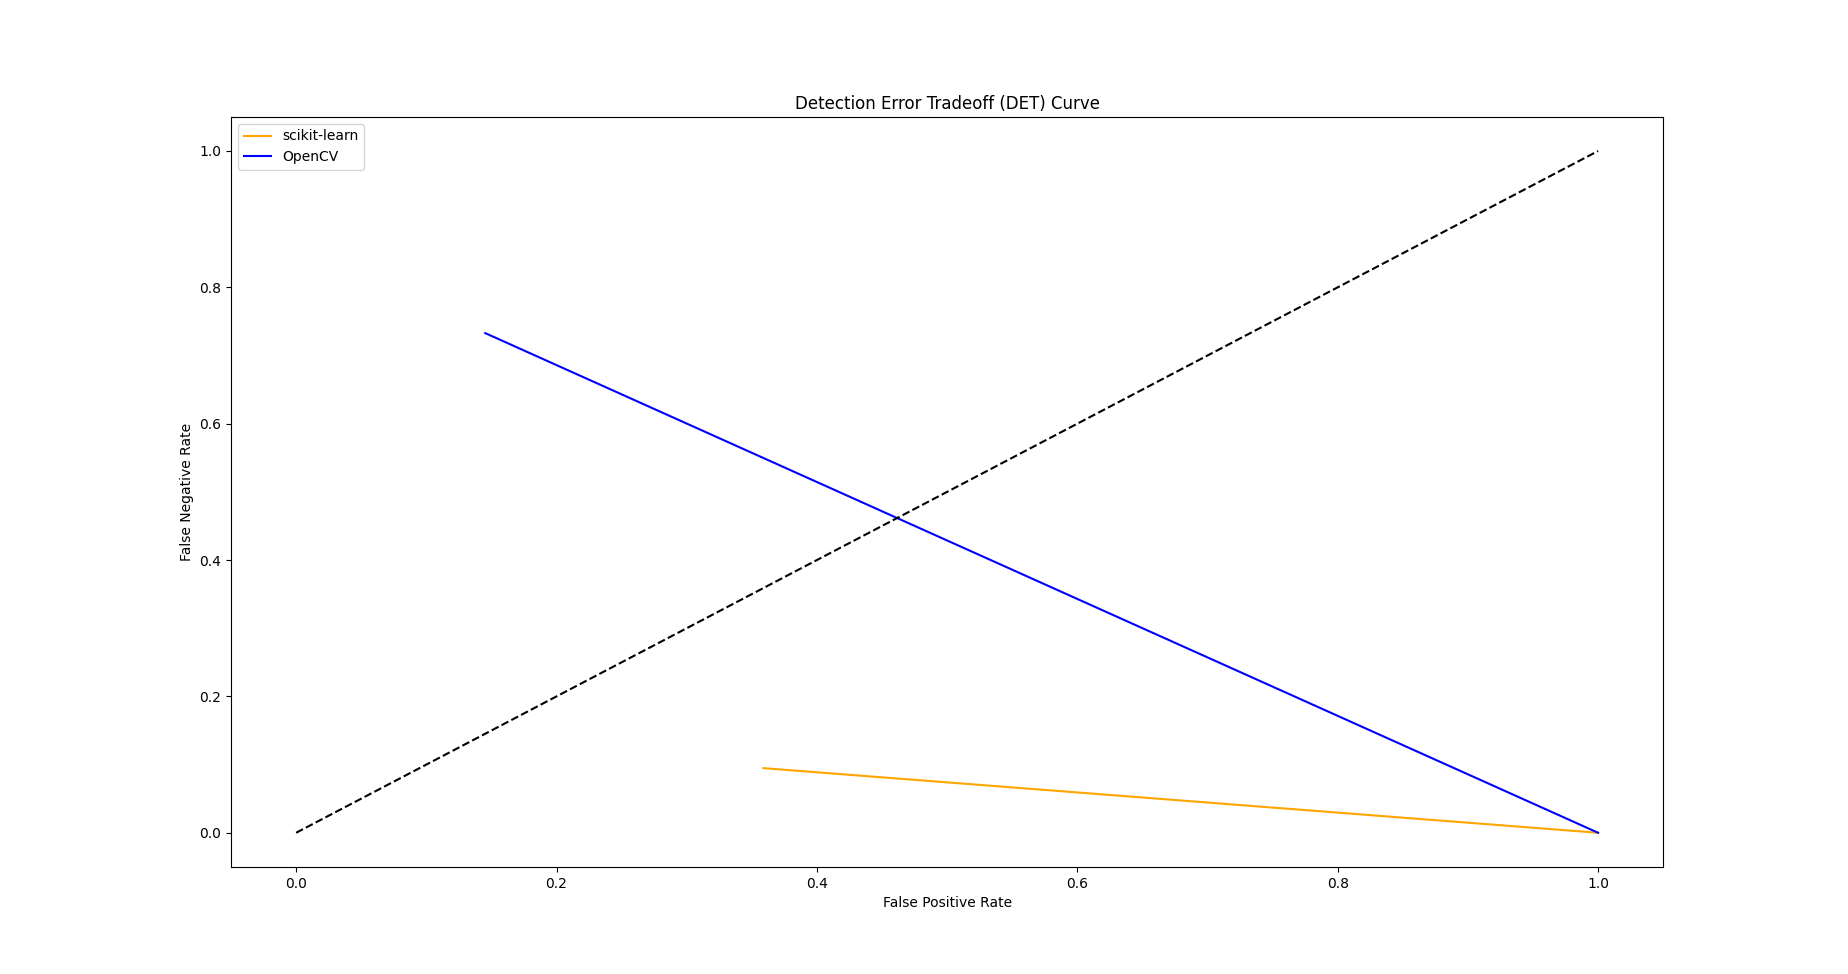
\includegraphics[scale=0.25]{images/det.png}
    \caption{DET.}
    \label{fig:det}
\end{figure}

On figure \ref{fig:eet} are plotted the false positive (i.e. false genuine) error rate and the false negative (i.e. false rejection) one, the intersection point is the equal error rate (EER), the ideal threshold seems to be 1.25.
Keep in mind that these two error rates are plotted against only three thresholds so this value is not necessary true. 
The EET is identified only for the scikit-learn SVM since it is the best model so far, for this same reason the online demo uses it.

\begin{figure}[h!t]
    \centering
    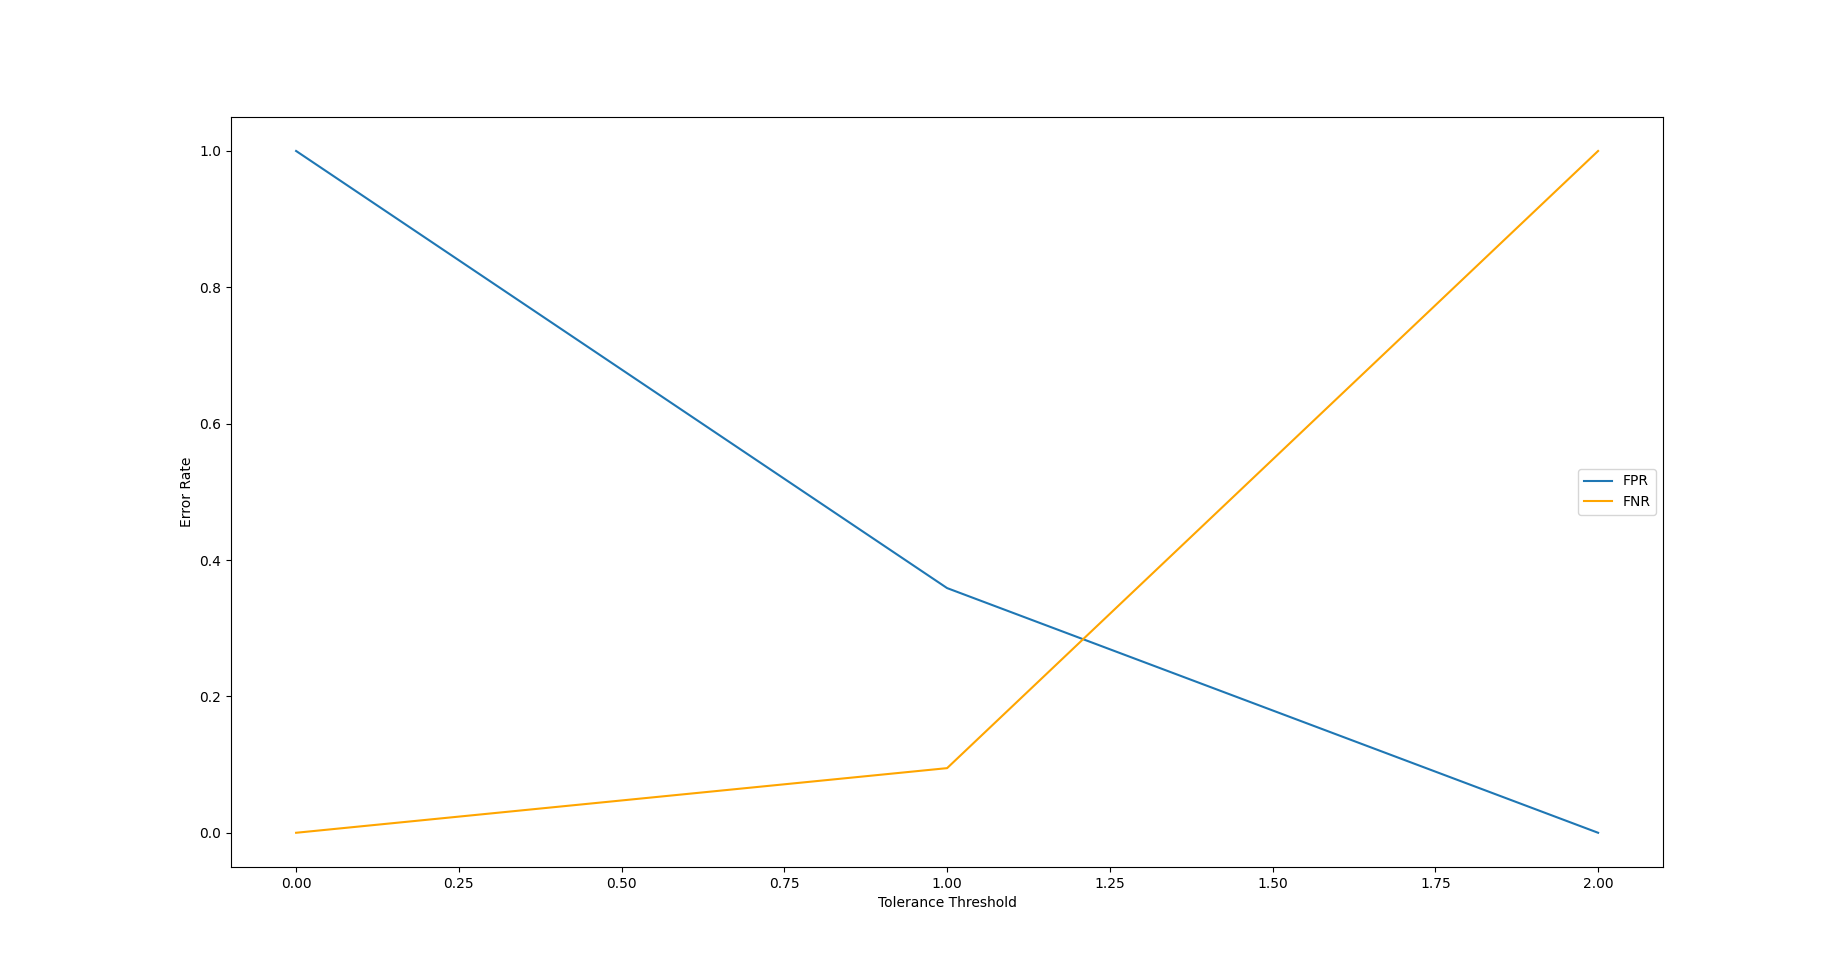
\includegraphics[scale=0.25]{images/eet.png}
    \caption{EET.}
    \label{fig:eet}
\end{figure}
